\documentclass{article}

\usepackage{fancyhdr} % Required for custom headers
\usepackage{lastpage} % Required to determine the last page for the footer
\usepackage{extramarks} % Required for headers and footers
\usepackage[usenames,dvipsnames]{color} % Required for custom colors
\usepackage{graphicx} % Required to insert images
\usepackage{listings} % Required for insertion of code
\usepackage{courier} % Required for the courier font
\usepackage{lipsum} % Used for inserting dummy 'Lorem ipsum' text into the template
\usepackage{amsmath}
\usepackage{titlesec}
\usepackage{pgfgantt}

\setcounter{secnumdepth}{4}

\titleformat{\paragraph}
{\normalfont\normalsize\bfseries}{\theparagraph}{1em}{}
\titlespacing*{\paragraph}
{0pt}{3.25ex plus 1ex minus .2ex}{1.5ex plus .2ex}

% Margins
\topmargin=-0.45in
\evensidemargin=0in
\oddsidemargin=0in
\textwidth=6.5in
\textheight=9.0in
\headsep=0.25in

\linespread{1.08} % Line spacing

% Set up the header and footer
\pagestyle{fancy}
\lhead{\hmwkAuthorName} % Top left header
\chead{Individual Project Specification and Plan} % Top center head
\rhead{December 9th 2015}
\lfoot{\lastxmark} % Bottom left footer
\cfoot{\ \thepage\ of\ \protect\pageref{LastPage}} % Bottom right footer
\renewcommand\headrulewidth{0.4pt} % Size of the header rule
\renewcommand\footrulewidth{0.4pt} % Size of the footer rule


%----------------------------------------------------------------------------------------
%	DOCUMENT STRUCTURE COMMANDS
%	Skip this unless you know what you're doing
%----------------------------------------------------------------------------------------

% Header and footer for when a page split occurs within a problem environment
\newcommand{\enterProblemHeader}[1]{
\nobreak\extramarks{#1}{#1 continued on next page\ldots}\nobreak
\nobreak\extramarks{#1 (continued)}{#1 continued on next page\ldots}\nobreak
}

% Header and footer for when a page split occurs between problem environments
\newcommand{\exitProblemHeader}[1]{
\nobreak\extramarks{#1 (continued)}{#1 continued on next page\ldots}\nobreak
\nobreak\extramarks{#1}{}\nobreak
}

\setcounter{secnumdepth}{0} % Removes default section numbers
\newcounter{homeworkProblemCounter} % Creates a counter to keep track of the number of problems

\newcommand{\homeworkProblemName}{}
\newenvironment{homeworkProblem}[1][Problem \arabic{homeworkProblemCounter}]{ % Makes a new environment called homeworkProblem which takes 1 argument (custom name) but the default is "Problem #"
\stepcounter{homeworkProblemCounter} % Increase counter for number of problems
\renewcommand{\homeworkProblemName}{#1} % Assign \homeworkProblemName the name of the problem
\section{\homeworkProblemName} % Make a section in the document with the custom problem count
\enterProblemHeader{\homeworkProblemName} % Header and footer within the environment
}{
\exitProblemHeader{\homeworkProblemName} % Header and footer after the environment
}

\newcommand{\problemAnswer}[1]{ % Defines the problem answer command with the content as the only argument
\noindent\framebox[\columnwidth][c]{\begin{minipage}{0.98\columnwidth}#1\end{minipage}} % Makes the box around the problem answer and puts the content inside
}

\newcommand{\homeworkSectionName}{}
\newenvironment{homeworkSection}[1]{ % New environment for sections within homework problems, takes 1 argument - the name of the section
\renewcommand{\homeworkSectionName}{#1} % Assign \homeworkSectionName to the name of the section from the environment argument
\subsection{\homeworkSectionName} % Make a subsection with the custom name of the subsection
\enterProblemHeader{\homeworkProblemName\ [\homeworkSectionName]} % Header and footer within the environment
}{
\enterProblemHeader{\homeworkProblemName} % Header and footer after the environment
}

%----------------------------------------------------------------------------------------
%	NAME AND CLASS SECTION
%----------------------------------------------------------------------------------------

\newcommand{\hmwkTitle}{Individual Project Specification and Plan} % Assignment title
\newcommand{\hmwkDueDate}{Wednesday, 9th December} % Due date
\newcommand{\hmwkClass}{Individual Project Specification and Plan} % Course/class
\newcommand{\hmwkClassTime}{} % Class/lecture time
\newcommand{\hmwkClassInstructor}{} % Teacher/lecturer
\newcommand{\hmwkAuthorName}{Paul McGurk} % Your name

%----------------------------------------------------------------------------------------
%	TITLE PAGE
%----------------------------------------------------------------------------------------

\title{
\textmd{\textbf{Individual Project Specification and Plan}}\\
}

\author{\textbf{\hmwkAuthorName}}

%----------------------------------------------------------------------------------------
\begin{document}
%\tableofcontents
\newpage
\section{Overview}
\subsection{Introduction}
The aim of this project is to provide an alternative way of gauging the current opinion on a lecture, as well as set questions, in a way which is easy and requires the least amount of dedicated hardware as possible. This is to reduce issues with current ``Classroom Clickers'', in that passing out the hardware and keeping track of them can be an issue with larger classes. They can also be expensive as lots of dedicated hardware is required. This reducement in dedicated hardware will be achieved by allowing any Wi-Fi direct enabled device to be used as the ``Clicker''.

It can also be used by the lecturer to ask simple questions, for example, multiple choice. This is to allow the lecturer to survey the general understating of the current topic, allowing them to tailor their lecturer accordingly.

Feedback will be given through two different ways. First of all, the screen that the lecturer uses to assign the questions (their laptop, the touchscreen on the dedicated hardware) will show an expanded version of the data. Secondly, there will be a simpled version of the data displayed to the whole class, most likely through the use of a ``Dotti''; a device with programmable LEDs, or through a device of my own creation.

\section{Requirements}
\subsection{Functional}
\subsubsection{Lecture Side Requirements}
\begin{enumerate}
	\item Must log in to system and access Lecturer interface.
	\item Must set questions.
	\item Must view responses to questions visualised in a clear way (Graphs, etc)
	\item Should customise question settings, such as: 
	\begin{enumerate}
		\item question visibility (Hidden, Public)
		\item answers options available (A, B, C, D or True/False, etc.)
		\item answers visibility (Shown after answer is given, or all users respond, etc)
	\end{enumerate}
	\item Could create ``Classes'' that contain questions.
	\item Could have the option to display the responses on a Dotti like device.
\end{enumerate}
\subsubsection{Student Side Requirements}
\begin{enumerate}
	\item Must answer questions.
	\item Must get feedback on answer depending on question settings.
	\item Must access Student interface.
	\item Should log in to system.
	\item Could join ``Classes'' owned by Lecturers.
\end{enumerate}

\subsection{Non-functional}
\begin{enumerate}
	\item Must be Accessible by users of all abilities and professions.
	\item Must be Usable in a classroom setting i.e. set up in the limited time of a lecture.
	\item Must be Secure enough to store users passwords, possible exam questions. Encrypted.
	\item Should be Cheap enough to be deployed throughout the campus.
	\item Should be Portable enough to be moved from classroom to classroom.
	\item Could be Flexible, as different courses have different questions.
\end{enumerate}
\section{Technology Used}
\subsection{Raspberry Pi}
A Raspberry Pi is a credit card-sized single-board computer developed by the Raspberry Pi Foundation. It is useful in this project as it is cheap, portable, and powerful enough to perform well enough to do what is required by this project. 

It will be used as a local Web server that hosts the web application and is accessible through connecting to it on a wi-fi direct enabled device.

\subsection{JavaScript and JQuery}
JavaScript is a client based, high-level programming language. It is used largely on Web Applications. JQuery is a framework for JavaScript which brings loads of additional features to it, including better mobile compatibility. 

This is what the main chunk project will largely be written in, using AJAX to send, and retrieve, data from the database.

\subsection{MySQL and PHP}
MySQL is a database management system. PHP is a backend language that works well with MySQL.

These will be used to store and access the various information required for the web application, such as Student accounts, Lecturer accounts, Questions, Classes, etc. 

\subsection{Materialize}
Materialize is a JavaScript framework, built heavily around JQuery, that allows users to create websites that follow the Google Material design. It also allows websites to be responsive depending on screen size, making it ideal for this application as it will be used over a range of devices.

This is used as the framework for the Web Application.

\subsection{Wi-Fi Direct}
Wi-Fi direct is a Wi-Fi standard that enables devices to connect and communicate without using a wireless access point. It communicates with more than one device simultaneously at Wi-Fi speeds.

This will be used to connect the various Wi-Fi direct enabled devices to the Raspberry Pi so the devices are able to access the local Web application files stored on the Pi.

\subsection{Technology Stack Diagram}
\begin{center}
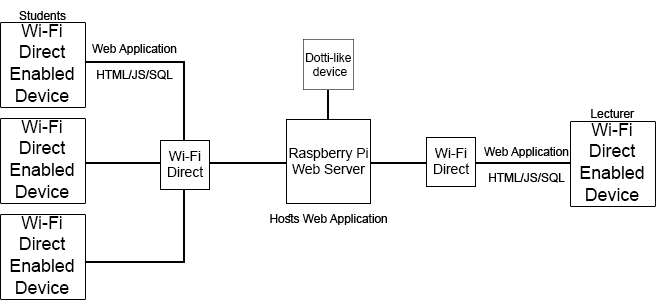
\includegraphics[width=0.8\textwidth]{stackdiagram.png}
\end{center}

\section{Software Development Process}
This web application with be implemented in a mixture of HTML5, CSS3 for the GUI, JavaScript for the client based functionality, PHP for the client to server communication and MySQL for the database functionality.

How this web application will be access is still under consideration, seeing as Wi-Fi direct has been difficult to set up in a way that is useful for this project. However, many alternatives are available, with some outlined in the ``Risks'' section of this report.

This should not affect the development of the web application, and the implementation of the functionality of the project will be the priority, with Wi-Fi direct, or alternatives to, will be investigated during this time as well.

\subsection{Example User Flow}
\begin{center}
    \center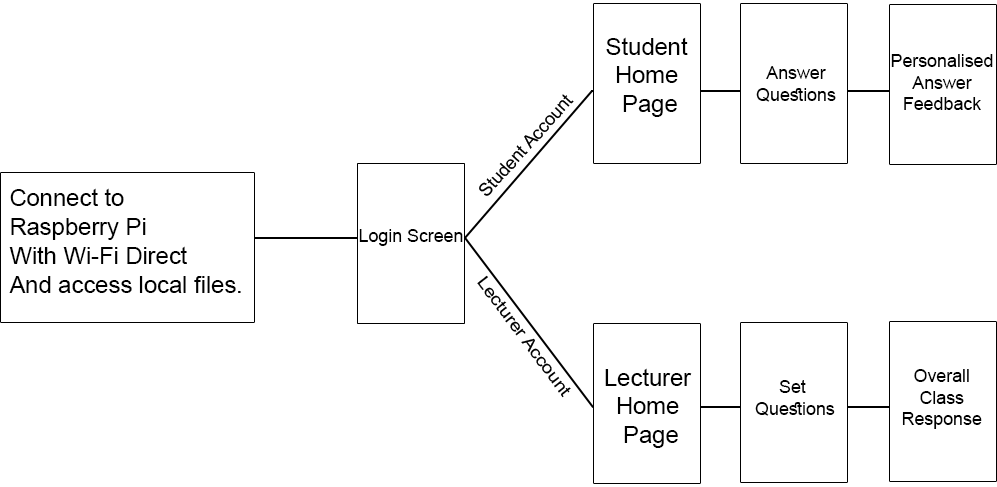
\includegraphics[width=0.8\textwidth]{userflow.png}
\end{center}

\section{Evaluation}
\subsection{Method}
Evaluation will involve a live preview of the system in the intended environment with the target end users; a lecturer and students. These users will be recruited by contacting lecturers and inquiring if it would be a system they would be interested in, with students in the class optionally choosing to use the system within the setting or not.

Participants will be expected to simply use the system in place of a normal class-room clicker, with questions being set by the lecturer and the students answering them on their Wi-Fi direct enabled devices. 

\subsection{Questionnaires}
\subsubsection{Students}
\begin{enumerate}
	\item General opinion on ``Classroom Clicker'' systems.
	\item Usability of the system (compared with previous similar systems, if used).
\end{enumerate}

\subsubsection{Lecturers}
\begin{enumerate}
	\item General opinion on ``Classroom Clicker'' systems.
	\item Usability of the system (compared with previous similar systems, if used).
	\item Likeliness of using system again as a learning tool.
\end{enumerate}
No personal information is required for this evaluation, and therefore will not be asked for.


\section{Risks}
\subsection{Wi-Fi Direct}
There is a possibility that Wi-Fi Direct will not be able to implement the idea of the application fully. This is due to the peer-to-peer nature of the standard, as well as the potential of lack of comparability with non-android phones. This is still under investigation at this point, with various alternative systems as a fallback, for example:
\begin{enumerate}
	\item Using the Raspberry Pi as a Wi-Fi access point to access the local Web server.
	\item Taking the Raspberry Pi out of the equation, and using a remote Web server for the Web application.
\end{enumerate}




\end{document}